\section{Experimental Settings and Evaluation}
All models, unless otherwise stated, are trained on data up to May 2018. Data from June 2018 is used for validation. The results are reported on the remaining months, i.e., August through October 2018. Note, Nov-Jan 2019 is not used for evaluation as these months only have ground-truth for Military Action events.

As stated in the previous sections, the machine learning models perform five micro-tasks in total - Event Detection, location identification, actor/target extraction, event-subtype identification, date extraction. For all micro-tasks, except for date extraction, the ML models can abstain from making a prediction. In such cases the document is sent for human supervision and the annotators are asked to provide an answer for that micro-task. Note the annotators only fill-in the information for the asked field (as defined by the micro-task) and do not change any other fields extracted by the ML models.

We report the performance of our overall system using the Performance metrics as defined by the IARPA OSI Mercury program. The performance metrics include -  
\begin{itemize}
    \item \textbf{Event Detection Performance Metrics}
    \begin{itemize}
        \item Precision/Recall/F1 metrics: These metrics are defined as expected and are standard.
\item Risk-Coverage Curve: Risk is defined as the percentage of false classifications (False Positives + False Negatives) w.r.t to the number of data points that are considered / covered. Coverage is defined as the percentage of data remaining after churning out documents on which the model score is less than the identified threshold. The curve is plotted by first sorting the model predictions in terms of its confidence score and moving the threshold from 0 to 100th percentile value of the confidence score. 
    \end{itemize}

\item \textbf{Event Encoding Performance Metrics}
    \begin{itemize}
        \item \textbf{Quality Score:} A score out of 4 and is a weighted sum over the extraction performance for each individual field in an event record. The performance for each field is a score between 0 and 1, with 1 indicating perfect extraction and 0 referring to fully wrong extraction. The components of QS are  
        % \textcolor{red}{Need to explain each individual score metric}
            \begin{enumerate}
                \item Actor score
                \item Target Target score
                \item Target Status score
                \item Location score
                \item Event Sub-type score
                \item Date score
            \end{enumerate}

         \item \textbf{Macro and Micro averages:} The macro and micro averages of the 
    above mentioned metrics are defined similar to the macro and micro averages in classification problems. For Macro-average, we first calculate QS, Precision, Recall and F-1 per document (i.e. the extracted events in a document are only evaluated against the ground-truth events in that document) and then take the average of the scores per document. 
    For Micro-average metrics, we evaluate all extracted events against all ground-truth events irrespective of which document they came from.
    \end{itemize}
\end{itemize}

\section{Results and Discussion}
In this section we will present the scores obtained by our event encoding system. Specifically we aim to answer the following major questions.

\begin{enumerate}
    \item What is the event detection performance of our AutoGSR system?
    \item How good is the uncertainty/confidence characterization of the event detection model?
    \item What is the performance of human annotators for each micro-task?
    \item How many documents are abstained per micro-task?
    \item What is the event extraction performance of the ML only System?
    \item What is the event extraction performance of the Hybrid System?
    \item What is the overall conclusion for performing MANSA event encoding?
    % \item What is the performance of our system in CU event encoding?
\end{enumerate}
In the following subsections we will look at each question individually.

\subsection{What is the event detection performance of the ML-only system?}
Here we present the performance of our ML system for the micro-task of event detection. The event detection micro-task involves predicting if an article contains an event or not. 

\begin{table}
    \centering
   \begin{tabular}{lrrrr}
\toprule
{} &  Precision &  Recall &    F1-score &  Support \\
\midrule
No-event            &  0.97 &   0.95 &  0.96 &   15843 \\
Event               &  0.75 &   0.84 &  0.79 &   2760 \\
micro avg           &  0.93 &   0.93 &  0.93 &   18603 \\
macro avg           &  0.86 &   0.90 &  0.88 &   18603 \\
weighted avg        &  0.94 &   0.93 &  0.94 &   18603 \\
\bottomrule
\end{tabular}
    \caption{Event Detection performance for English documents in test set.}
    \label{tab:engDetection}
\end{table}


\begin{table}
    \centering
   \begin{tabular}{lrrrr}
\toprule
{} &  Precision &  Recall &    F1-score &  Support \\
\midrule
No-event            &  1.0 &  1.00 &  1.00 &  28643 \\
Event               &  1.0 &  0.36 &  0.53 &   73 \\
micro avg           &  1.0 &  1.00 &  1.00 &  28716 \\
macro avg           &  1.0 &  0.68 &  0.76 &  28716 \\
weighted avg        &  1.0 &  1.0  &  1.00 &  28716 \\
\bottomrule
\end{tabular}
    \caption{Event Detection performance for Arabic documents in test set.}
    \label{tab:arDetection}
\end{table}

The tables Tab.~\ref{tab:engDetection} and ~\ref{tab:arDetection} provides the performance metrics our event detection system for English (Tab.~\ref{tab:engDetection}) and Arabic documents (Tab.~\ref{tab:arDetection}) for the test period.

We note that the performance of event detection is better in English than Arabic. However, it is to be noted that for Arabic, the event detection task is extremely imbalanced (the ratio of positive documents is 0.2\% vs 14.8\% for English). 


\subsection{How good is the uncertainty/confidence characterization of the event detection model?}
As mentioned above, the confidence score of  the event detection is taken to be the predicted probability of the max class. Figure.~\ref{fig:engPrec} gives the precision vs confidence plot for English documents and Figure.~\ref{fig:arPrec} for Arabic documents.

\begin{figure}
    \centering
    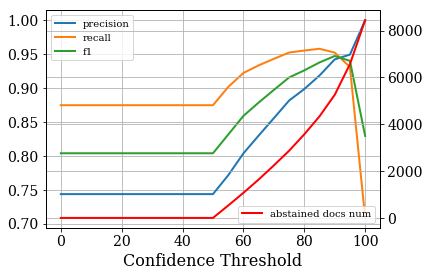
\includegraphics[width=0.6\textwidth]{figures/english_precConf.png}
    \caption{Precision vs Confidence plot for English. The right-side axis denotes the number of documents that will be abstained at the current threshold}
    \label{fig:engPrec}
\end{figure}

\begin{figure}
    \centering
    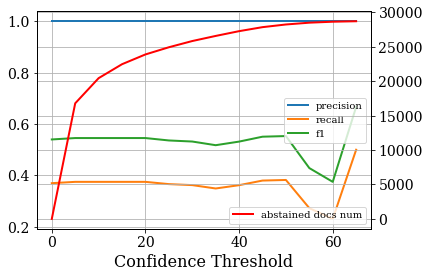
\includegraphics[width=0.6\textwidth]{figures/arabic_precConf.png}
    \caption{Precision vs confidence plot for Arabic}
    \label{fig:arPrec}
\end{figure}

From Figure.~\ref{fig:engPrec}, we can see that Precision, Recall, F-1 metrics increase almost uniformly as the confidence threshold is increased. The Recall and F-1 metrics fall sharply for high values of the threshold.
However for Arabic (From Figure.~\ref{fig:arPrec}), there isn’t much performance improvement achieved by thresholding on the confidence.

Another way at quantifying uncertainty of the classification model would be to look at the area under the Risk-Coverage (RC) curve. Figure.~\ref{fig:engRisk} provides the RC curve for English and Arabic.
\begin{figure}
    \centering
    \begin{subfigure}[b]{0.45\textwidth}
         \centering
         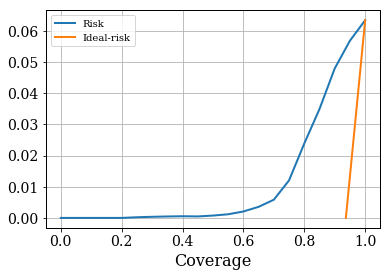
\includegraphics[width=\textwidth]{figures/english_riskCoverage.png}
         \caption{}
         \label{fig:engRisk}
    \end{subfigure}
    \hfill
    \begin{subfigure}[b]{0.45\textwidth}
         \centering
         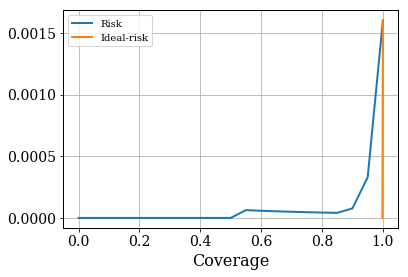
\includegraphics[width=\textwidth]{figures/arabic_riskCoverage.png}
         \caption{}
         \label{fig:y equals x}
     \end{subfigure}
     \caption{Risk-coverage curve for (a) English and (b) Arabic. The orange curve represents the ideal-risk i.e., the risk when the classifier is correctly calibrated
 ($\textrm{loss}(x_i) > \textrm{loss}(x_j) \textrm{, iff conf}(x_j) < \textrm{conf}(x_i))$}
\end{figure}

We notice from Figure.~\ref{fig:engRisk} that the risk drops to almost zero at about 50\% coverage. Note Risk is defined as the percentage of False classifications.



\subsection{What is the performance of human annotators for each micro-task?}
For estimating the performance of each human annotator, we randomly chose a micro-task for a given document and asked the annotator to provide encoding for the field denoted by the micro task. For each micro-task, the annotators were shown the encoding of the remaining fields, however they were not allowed to change these fields.

The pie chart shown in Figure.~\ref{fig:microTimings} gives the time distribution (in seconds) per micro-task. The time per task reported here is the average of the median time taken by each annotator. The median is taken after removing the top and bottom 10 percentile of times of an annotator. This is done to remove anomalous records (For example, cases where the annotator simply leaves the autogsr web-page on without logging off.)

\begin{figure}[h!]
    \centering
    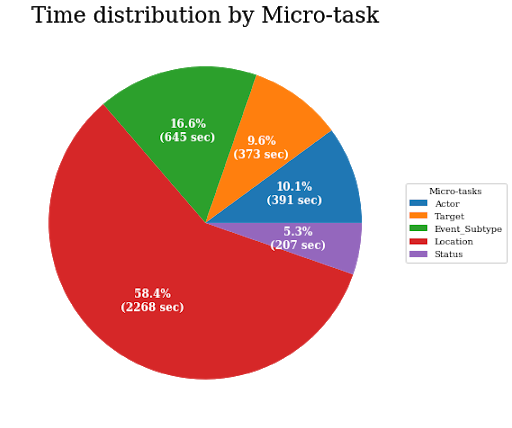
\includegraphics[width=0.5\textwidth]{figures/micro_task_timings.png}
    \caption{Average time spent per document per microtask by an annotator}
    \label{fig:microTimings}
\end{figure}

Figure.~\ref{fig:microTimings} shows the human annotators spent maximum time (58.4\%, ~approx 37 minutes) in encoding the location of the events. The least amount of  time was spent on  identifying the status of the article. Note status here refers to the event detection task.  The average accuracy per micro-task across all annotators is provided in Figure.~\ref{fig:microPerf}. We can see that the annotators have difficulty in identifying the status of an article.


\begin{figure}[h!]
    \centering
    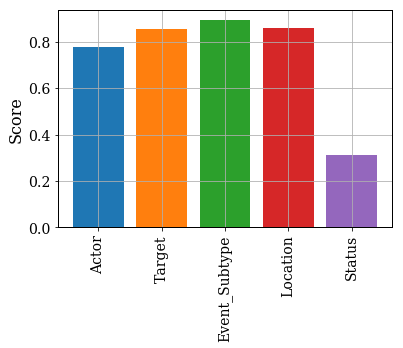
\includegraphics[width=0.5\textwidth]{figures/micro_task_performance.png}
    \caption{Average accuracy of human annotators on micro-tasks}
    \label{fig:microPerf}
\end{figure}

\subsection{How many documents are abstained per micro-task by the ML system?}
\begin{table}[]
    \centering
    \small
    \begin{tabular}{l|r}
    \toprule
       \textbf{Micro-Task}  & \textbf{\#Abstained Documents} \\
    \midrule
       Event Detection &  1936 / 57401 (3.00\%) \\
       Location  & 307/2137 (14.3\%) \\
       Actor/Target & 1002/2137 (46.8\%) \\
       All (Location, Actor, Subtype) & 320/2137 (14.9\%) \\
    \bottomrule
    \end{tabular}
    \caption{Documents sent for human supervision}
    \label{tab:abstPerMicro}
\end{table}



In this section we discuss the number of documents the ML system abstained from making a prediction for each micro-task. The threshold for abstention for different micro-tasks was identified based on the validation set performance.  The threshold for event detection for Table.~\ref{tab:abstPerMicro} summarizes the number of documents we sent for human supervision for each micro-task

\subsection{What is the event coding performance of the ML only System?}
\begin{table}
\centering
\begin{tabular}{l|r|r}
\toprule
             Metrics &    Macro-avg &    Micro-avg \\
\midrule
               \#docs &   888 &   888 \\
 \# GroundTruthEvents &  2039 &  2039 \\
   \# ExtractedEvents &  1981 &  1981 \\
         Actor Score &     0.373888 &     0.602880 \\
          Date Score &     0.940764 &     0.840740 \\
 Event Subtype Score &     0.449895 &     0.680532 \\
      Location Score &     0.866620 &     0.800837 \\
 Target Target Score &     0.662297 &     0.677204 \\
 Target Status Score &     0.590778 &     0.828618 \\
           Precision &     0.691522 &     0.949447 \\
              Recall &     0.720177 &     0.891757 \\
       Quality Score &     2.774264 &     2.999131 \\
\bottomrule
\end{tabular}
\caption{Performance metrics of ML only system}
\label{tab:mlPerformance}
\end{table}
The table.~\ref{tab:mlPerformance} provides the quality scores of the events extracted from the machine learning model in the un-abstained set  (i.e from documents that are not sent for human supervision). Note we score events extracted from a document only against the ground-truth events from that document. For overall precision and recall we average precision and recall for each individual document. 

We can see from Table.~\ref{tab:mlPerformance} that the ML only system is very good at location and date extraction. The system does not perform well on  Actor identification. On further investigation of the events extracted by the ML system we found that the ML system is not able to distinguish between the different state actors of a given country. For example, ML model is not able to differentiate between “Iraqi Special Forces” and “Iraqi Security Forces” or “Iraqi Intelligence Service”.  We thus performed another evaluation after combining all state actors belonging to a country into a single entity. That is, we group all state actors of a country like “Iraq Security Forces”, “Iraqi Intelligence Service” , “Iraqi Police”, “Baghdad International Airport Security”, “Iraqi Military” and “Iraqi Special Forces” into one single entity  “Iraqi State Actors”.  The performance of our system after this correction is shown in Table.~\ref{tab:mlgrouped}.
\begin{table}
\centering
\begin{tabular}{lrr}
\toprule
              Metric &    Macro-avg &    Micro-avg \\
\midrule
               \#docs &   888 &   888 \\
 \# GroundTruthEvents &  2039 &  2039 \\
   \# ExtractedEvents &  1981 &  1981 \\
         Actor Score &     0.551631 &     0.727570 \\
          Date Score &     0.940403 &     0.842904 \\
 Event Subtype Score &     0.451160 &     0.682170 \\
      Location Score &     0.867125 &     0.805017 \\
 Target Target Score &     0.588879 &     0.677740 \\
 Target Status Score &     0.661664 &     0.822260 \\
           Precision &     0.691522 &     0.951026 \\
              Recall &     0.720177 &     0.893247 \\
       Quality Score &     2.892902 &     3.087752 \\
\bottomrule
\end{tabular}
\caption{Performance metrics of ML only system with different state actors of one country grouped into one entity}
\label{tab:mlgrouped}
\end{table}


\subsection{What is the event coding performance of the hybrid system?}
\begin{table}[]
    \centering
    \begin{tabular}{lrr}
\toprule
              Metric &    Macro-avg &    Micro-avg \\
\midrule
               \#docs &  2137 &  2137 \\
 \# GroundTruthEvents &  4265 &  4265 \\
   \# ExtractedEvents &  4239 &  4239 \\
         Actor Score &     0.621032 &     0.755090 \\
          Date Score &     0.952899 &     0.878390 \\
 Event Subtype Score &     0.539359 &     0.646776 \\
      Location Score &     0.926107 &     0.838040 \\
 Target Target Score &     0.680881 &     0.703337 \\
 Target Status Score &     0.727046 &     0.828054 \\
           Precision &     0.791948 &     0.946720 \\
              Recall &     0.819668 &     0.915887 \\
       Quality Score &     3.121909 &     3.161470 \\
\bottomrule
\end{tabular}
    \caption{Performance metrics of the hybrid system for MANSA Event Encoding}
    \label{tab:hybridPerf}
\end{table}
Table.~\ref{tab:hybridPerf} provides the event extraction performance for the Hybrid system. The hybrid system includes predictions from the ML system along with inputs from human annotators for the micro-tasks on documents where the ML system was not confident on.


\subsection{What is the overall Conclusion for creating a MANSA event encoding system?}
From Tables.~\ref{tab:mlPerformance} and ~\ref{tab:mlgrouped} we can see that the ML models performs well in identifying Location, Date, and event status as compared to the human annotators. The human annotators on average perform better than the ML model on Actor and Target identification. 
A viable system could be one where the ML system performs the location, date and status identification and human annotators provide the actor/target extraction. The human annotators on average take approximately 12.6 minutes per document for actor and target identification and have an accuracy of approx ~80\% for the extraction of the two fields.  So for a dataset similar to our test set, we would need approximately 448.77 man hours.


% \subsection{What is the  performance of our system in CU event encoding?}
% For Civil Unrest, we train all our models on data obtained from the EMBERS autogsr system. And for testing we use the CU event articles from the CFA dataset. This experimental setting was chosen due to the presence of only a few articles with CU events in the CFA dataset.

% Table 8 provides the event detection performance for Civil Unrest. 

